\chapter{Conclusions}
\label{cha:conclussions}

En aquest cap\'{i}tol es descriu la evolució temporal, la gestió del projecte, la estimació econòmica resultat i les possibles millores que es poden realitzar. Per finalitzar, plantejo en forma de reflexió personal les conclusions de la realització d'aquest projecte.


\section{Metodologia àgil}
Per la realització del projecte s'han emprat una metodologia \textit{agile}. Concretament aprofitant tècniques i artefactes de l'SCRUM.\cite{agile}\\

Els principis bàsics de la metodologia àgil són\cite{agilemanifesto}:
\begin{itemize}
\item Els individus i les seves interaccions per sobre dels processos i les eines.
\item El programari que funciona per sobre de la documentació exhaustiva.
\item La col·laboració amb el client per sobre de la negociació de contractes.
\item La resposta davant del canvi per sobre de seguir un pla tancat.
\end{itemize}

Per la realització d'aquest projecte s'han realitzat iteracions quinzenals amb el \textit{product owner}}.\cite{productowner} En cada iteració s'han anat canviant requisits, analitzant tecnologies, definint noves especificacions, definint nous requisits i fent petites \textit{demos} dels avanços implementats en cada iteració.\\

\subsection{Backlog}
En el cas d'aquest projecte s'ha usat l'artefacte principal ''Backlog'' mitjançant histories de usuaris. Les historia d' usuari son una una representació d'un requisit del \textit{software} escrit en una o dos frases. En aquest cas:\\

\centerline{Com \textbf{rol} vull fer \textbf{alguna cosa} per \textbf{obtenir benefici}}
~\\
A la taula \ref{table:backlog} es pot veure el \textit{backlog} amb les histories d'usuaris puntuant cadascuna segons la serie de Fibonnaci.\cite{backlogfibonnacci}. Eludim els requeriments ja que es poden consultar al capítol \ref{cha:specification}.

\begin{center}
\begin{longtable}{ | p{3cm} | p{5cm} | p{5cm} | p{1cm} | }
\hline
\multicolumn{1}{|c|}{\textbf{Com}} & \multicolumn{1}{|c|}{\textbf{vull}} & \multicolumn{1}{|c|}{\textbf{per}} &\multicolumn{1}{|c|}{\textbf{Punts}} \\ \hline
Usuari anònim &	registrar-me &	usar la aplicació &	3 \\ \hline
Usuari registrat &	recuperar el password & entrar en cas que m'ho oblidi de la contrasenya & 3 \\ \hline
Usuari administrador &	vull afegir variables & indicar en les matrius quina variable de Ichnaea representa & 1 \\ \hline
Usuari registrat &	crear una matriu important un csv o excel & configurar-la i crear entrenaments & 8 \\ \hline
Usuari registrat &	crear un entrenament a partir d'una matriu & crear prediccions & 5 \\ \hline
Propietari d'una matriu & configurar una matriu & executar un entrenament & 21 \\ \hline
Propietari d'una matriu	& esborrar una matriu & eliminar dades, entrenaments i prediccions & 3 \\ \hline
Usuari registrat &	crear una predicció important un csv o excel & crear un conjunt de dades per predir i executar-es a Ichnaea & 8 \\ \hline
Propietari d'entrenament & 	esborrar una predicció & eliminar dades i prediccions & 2 \\ \hline
Usuari registrat & veure els resultat d'una predicció & consultar dades i crear una predicció & 1 \\ \hline
Usuari registrat & vull veure les matrius del sistema creades publiques & crear entrenaments a partir d'elles & 2  \\ \hline
Usuari registrat & vull veure els entrenaments finalitzats correctament	 & crear prediccions a partir d'elles & 2  \\ \hline
Usuari registrat & vull afegir conjunts de fitxers a un variable & indicar en les matrius quina conjunt de fitxers enviar a Ichnaea & 3  \\ \hline
Usuari registrat & vull esborrar fitxers d'un conjunt de fitxers & corregir dades en cas d'errors & 2 \\ \hline
Usuari administrador & vull testejar el sistema de cues & assegurar el correcte funcionament amb el sistema de cues en cas de detectar errors d'accesibilitat & 1 \\ \hline
Sistema de cues & vull indicar al sistema web que he acabat un entrenament & actulitzar les dades d'un entrenament i guardar els resultats al disc & 5 \\ \hline
Usuari registrat & enviar un predicció a la cua d'execucions de prediccions & predir origens de mostres & 5  \\ \hline
Usuari registrat & veure els resultats d'una predicció & consultar dades predites & 3  \\ \hline
Usuari registrat & veure un entrenament & consultar les dades entrenades i crear un predicció & 2  \\ \hline
Propietari d'un entrenament & vull enviar un entrenament a execució & poder crear prediccions & 5  \\ \hline
Sistema de cues & indicar al sistema web que tinc un resultat & poder consultar prediccions & 3  \\ \hline
Propietari d'una predicció & configurar les dades d'una matriu	& enviar les dades a Ichnaea per predir & 21  \\ \hline
Propietari d'una matriu & validar la matriu	 & comprovar la validessa de les dades & 5  \\ \hline
\caption{Taula de \textit{backlog} ponderada amb la serie de Fibonnaci}
\label{table:backlog}
\end{longtable}
\end{center}

\section{Planificació}
A la figura \ref{fig:gant} es descriu la planificació àgil per setmanes i per ítems.\\
\begin{sidewaysfigure}[ht]
    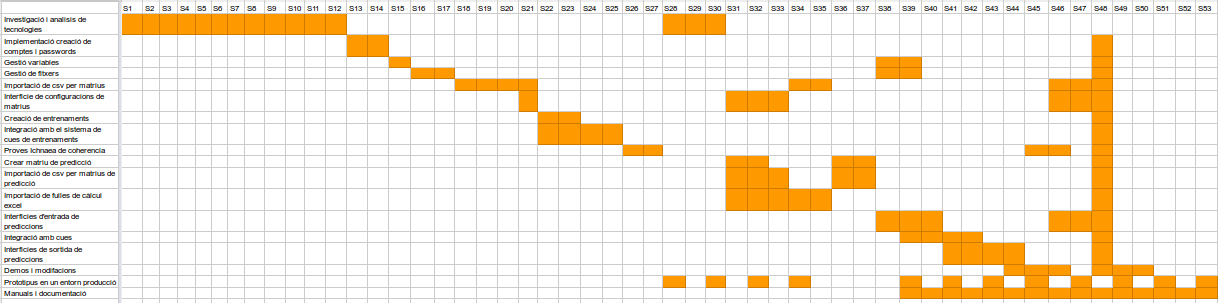
\includegraphics[scale=0.5]{img/conclussions/gantz.png}
    \caption{Diagrama de Gant de planificacio del projecte}
    \label{fig:gant}
\end{sidewaysfigure}

Al contrari de les metodologies en cascada, a on no es passa al següent ítem fins que s'acabi, es pot veure com es modifiquem ítems anteriors segons els canvis en cada iteració \textit{agile}.

\section{Estimaci\'{o} econ\'{o}mica}
La estimació del cost es calcula tenint en compte els següents paràmetres i consideracions:
\begin{itemize}
\item Cada setmana de desenvolupament del projecte son 15 hores
\item C\`{a}lcul a partir del cost. Es contempla com a cost intern seguint el cost dels rols involucrats en cada àrea.
\item C\`{a}lcul de venta com a servei. Es contempla el cas de venta de projecte com empresa segons els preus de mercats d'una consultoria \textit{StartUp} de desenvolupament a mida.
\item Es un projecte àgil. Tots els integrants treballen en totes les tareas.
\item Son iteracions r\'{a}pides de dues setmanes.
\end{itemize}

A la taula \ref{costs} a la p\`{a}gina \pageref{costs} s'especifiquen els costos resultats tenint en compte l'esmentat anteriorment.

\begin{sidewaystable}
\begin{tabular}{|p{2.75cm}|p{2cm}|p{1cm}|p{3cm}|p{1cm}|p{2cm}|p{2cm}|p{2cm}|p{1.75cm}|}
\hline
Tarea & Setmanes & Hores & Rols & Cost \euro/h & Cost total & Servei \euro/h & Servei total & Rendiment \\ \hline
Especificacions i tomes de requeriments & N/A: 3 hores per iteració & 91.5 h & Cap de projecte & 18 \euro/h & 1647\euro & 45 \euro/h & 4117.5\euro & \\ \hline
Anàlisis de tecnologia & 15 setmanes & 225 h & Analista & 15 \euro/h & 3375\euro & 30\euro & 6750\euro & \\ \hline
Implementació Aplicació & 32 setmanes & 480 h & Desenvolupador & 12 \euro/h & 5760 & 30\euro/h & 14440\euro & \\ \hline
Documentació i Qualitat & 14 setmanes & 210 h & Becari & 8 \euro/h & 1680\euro & & & \\ \hline 
\hline
Total & 61 setmanes & 1006.5 h & & & 12462\euro & & 25267.5\euro & 12805.5\euro \\ \hline
\end{tabular}
\caption{Taula de costos de la realització del projecte}
\label{costs}
\end{sidewaystable}


\section{Conclusions finals}
La realització d'aquest projecte est\'{a} motivada per la evolució d'Ichnaea com a sistema complexe. Durant l'us de la pròpia aplicació executant Ichnaea s'han pogut observar les millores que s'haurien de portar a terme al propi \textit{software} Ichnaea.\\

A m\'{e}s a m\'{e}s, durant les nostres reunions personals amb tots els involucrats s'han plantejat possibles millores conceptuals per continuar evolucionant Ichnaea, que no haguessin sortit si no fos per la implementació d'aquest projecte. 

\subsection{Millores per futures versions}
A continuació exposo un conjunt de possibles millores per una segona iteració del projecte.

\paragraph*{Personalitzaci\'{o} dels perfils d'usuari} Actualment els perfils d'usuari son dades basiques com noms, noms d'usuari i/o contrasenyes encriptades juntament amb processos per administrar aquestes dades com reenviar una contrasenya. Una millora interessant seria afegir dades configurables per l'usuari com, per exemple, en quin forma voldrien veure les dades de les matrius(exponencials o decimals) o en quin format volen establir les dates de les mostres.

\paragraph*{Internalització de l'aplicació} La internalització de les aplicacions \'{e}s un projecte sencer. Empreses tenen equips sencer d'enginyers per portar a terme aquestes tasques. Per exemple: traduccions, formats de dates, alfabets(ciríl·lic, àrab, xines,..), formats de decimals son algunes de les tasques que realitzen aquests equips i que es podria implementar en aquest projecte. 

\paragraph*{Ampliaci\'{o} de les API Restful} Actualment s'ha desenvolupat el motor dels serveis webs. Una ampliacio d'aquesta API seria interessant per desenvolupar aplicacions mòbils.

\paragraph{Depuraci\'{o} en entorn distribuït} Encara que la aplicaci\'{o} ha sigut desenvolupada per ser distribuïda i separada del sistema de cues, no ha sigut possible provar-la en un entorn m\'{e}s complexe i distribuït per falta de recursos.

\paragraph{Sistema de notificacions} Elaborar un sistema m\'{e}s el.laborat de notificacions per gestionar una bona comunicació amb l'usuari. Per exemple, notificacions quan un entrenament ha acabat o enviar correus electrònics per notificar als usuaris creadors de entrenaments o de prediccions en resposta a un esdeveniment de finalitzaci\'{o} d'algun d'aquests. 

\paragraph{Sistema de projectes} La aplicaci\'{o} no ha sigut contemplada per ser m\'{e}s col.laborat-iva. Hauria de ser m\'{e}s concurrent contra alguns recursos, com per exemple permetre diversos editors d'una matriu al mateix temps.

\paragraph{Sistema de invitacions} Un sistema per invitar col·laboradors a gestionar matrius, crear entrenaments i/o prediccions tant siguin usuaris ja registrats de la plataforma com si fossin externs.

\paragraph{Implementar tests autom\'{a}tics} Per aplicar metodologies de desenvolupament m\'{e}s robustes com per exemple TDD.\cite{tdd}

\subsection{Reflexió final}
Una millora conceptual que penso per una propera iteració es afegir una capa abstracte lògica m\'{e}s a la aplicació. Actualment el projecte ha sigut enfocat a la execució d'Ichnaea com a \textit{software}. Es a dir, purament exfocat als processos. Un concepte interessant seria tenir tot un repositori d'entrenaments i afegir una lògica de negoci per damunt per gestionar-los. Tenint aquest repositoris, l'aplicació podria estar enfocada a les prediccions i les localitzacions. Aquesta millora conceptual es completament escal.lable a aquest projecte. Justament aquest projecte i el model de dades implementat podria ser el motor d'aquesta nova capa. Un benefici d'aquesta millora seria la seguent situacio.

Imaginem un conjunt d'usuaris amb una aplicació mòbil entressin mostres de dades per fer prediccions a un pais X. Amb el GPS es donaria una localització i amb el rellotge es definís la data de la mostra en cadascuna de les mesures que els usuaris entressin. Aquesta millora podria anar fent prediccions, decidint quin entrenament usar sense especificar-lo. En el cas que no estigues entrenada i que tingues els envelliments per aquest pais i d'aquesta epoca de l'any decidiria crear un nou entrenament. I en el cas que no tingues res, notificaria als administradors per que intentessin definir envelliments per aquesta localització.\\

Encara que arribar fins aquest sistema esta lluny, ja es comença a discernir el potencial del sistema i de la evolucio que ha començat amb aquest projecte. El projecte es troba purament en l'àmbit de la investigació i no hi ha res semblant. Per tant ha sigut una oportunitat haver aportat un gra de sorra en aquest àmbit. I de tant segur acabara sent una eina per a els biòlegs ja que les expectatives son grans i ja tenim feina definida per a futures evolucions.\\

\'{E}s una gran experiència haver treballat i, sobretot, apres amb Lluís Belanche i Miguel Ibero. Han sorgit idees i hem resolt situacions per poder evolucionar aquest \textit{software} tan prometedor per intentar solucionar un problema que pot ser molt útil a la humanitat.